\section{Recherche de solution}

\subsection{L'algorithme de Canny}

\subsubsection{Version de base}
Le filtre de Canny a été créé en 1986 dans le but d'améliorer les résultat du filtre de Sobel.
Le principe du filtre est d'utiliser deux seuil, un seuil haut et un seuil bas. L'algorithme
commence par séléctionner les pixels supérieur au seuil haut, puis recherche à partir de chaque
pixels au dessus du seuil haut les pixels qui sont au dessus du seuil bas dans son voisinage. 
Chaque voisin qui est entre les deux seuils appartient à un contour, on passe donc sa valeur à
255 pour le prendre en compte dasn le contour. Ainsi on voit 
que cet algorithme prend en compte deux caractèristiques, l'intensité et la direction des 
gradients.\\

Nous utilisons cette algorithme dans les régions autour des yeux afin de délimiter le contour
de chaque oeil. Le résultat permet de faire ressortir l'oeil, mais aussi les sourcils et certaines
ombres présentent dans le creu de l'oeil. Ce filtre permet donc de détecter les contours des yeux,
mais le résultat comporte soit beaucoup de bruit, soit trop peu de détails. Dans un premier
temps, pour obtenir un seuil adaptatif, nous prenons la moyenne des pixels.

\begin{figure}[H]
 \center
 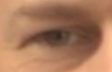
\includegraphics[width=4cm]{image/original.png}
 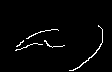
\includegraphics[width=4cm]{image/canny_moyenne.png}
 \caption{Image de test et résultat de l'algorithme de Canny avec une moyenne des pixels}
\end{figure}

On voit que cette méthode, n'est pas optimal et supprime beaucoup trop d'information. De plus,
l'algorithme prend beaucoup trop en compte les ombres présentent dans l'image.

\subsubsection{Avec une moyenne de pixels sur des parties d'image}

Plutôt, que de prendre la moyenne sur l'image de la zone périoculaire, nous segmentons l'image
en plusieurs zones dans lesquel nous calculons la moyenne et ou nous effectuons l'algorithme
de Canny.

\begin{figure}[H]
 \center
 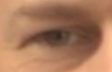
\includegraphics[width=4cm]{image/original.png}
 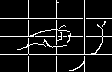
\includegraphics[width=4cm]{image/canny_decomposition.png}
 \caption{Image de test et résultat de l'algorithme de Canny avec division de l'image en 16}
\end{figure}

Avec cette méthode, nous obtenons une image bruité avec les bords de chaque rectangle utilisé
pour le calcul précédent, car l'algorithme de Canny ne prend pas en compte les bords de l'image
qu'il traite. Avec ce bruit nous ne pouvons clairement pas effectuer une recherche de l'oeil dans
l'image.

\subsubsection{Ouverture des sous-images}

La dilatation d'une image est une opération morphologique\footnote{filtre non-linéaire} qui pour chaque
pixel de celle-ci, remplace la valeurs des pixels voisin du pixel traité par la valeur de celui-ci.
Cette opération à en général pour effet d'élargir une forme et de combler les trous qui peut y avoir
dans cette forme. Nous avons également l'opération inverse qui est l'érosion, qui va rétrécire la forme.\\

L'ouverture est la combinaison des deux opérations morphologique vu précédemment, en commençant par 
l'érosion puis la dilatation. Cela à pour effet de fusionner des formes si elles sont proches (dans ce
cas il y a des chances que se soit la même forme) et de diminuer la largeur de la forme pour 
s'approcher de la forme réel. Afin de supprimer le bruit présent dans le résultat précédent nous effectuons une ouverture
de chaque sous-image.

\begin{figure}[H]
 \center
 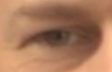
\includegraphics[width=4cm]{image/original.png}
 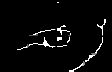
\includegraphics[width=4cm]{image/canny_final.png}
 \caption{Image de test et résultat de l'algorithme de Canny avec dilatation puis érosion des sous-images}
\end{figure}

Grâce à ce procédé, nous obtenons une image sans la grille que nous avions précédemment. Cependant,
le bruit du aux ombres et au ride ne permet pas encore d'effectuer un algorithme de détection de forme
sur l'oeil. Afin de supprimer les bruits du à l'ombre, nous décidons de travailler sur d'autre modèle
colorimètrique comme le HSV\footnote{Hue Saturation Value} dont la composante \enquote{saturation} peut nous
permettre de diminuer l'ombre de l'image.

%TODO mettre la méthode avec le masque

%\subsubsection{Avec égalisation d'histogramme}
% L'égalisation d'histogramme est un procédé qui essaye de placer le même nombre de pixels
% sur chaque composante de gris. Ce qui a pour effet d'augmenter le contraste de l'image
% et devrait ainsi améliorer les hautes fréquences de l'image, donc les contours. Nous avons
% essayé d'appliquer cette méthode sur une image en niveau de gris avant de lancer l'algorithme
% de Canny.
%TODO ajout des images

% \subsection{Normalisation et égalisation d'histogramme}
% 
% \begin{figure}[H]
%  \center
%  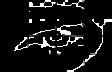
\includegraphics[width=4cm]{image/normalisation.png}
%  \caption{Algorithme de Canny après normalisation de l'histogramme de l'image de gris}
% \end{figure}
% 
% \begin{figure}[H]
%  \center
%  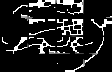
\includegraphics[width=4cm]{image/egalisationHist.png}
%  \caption{Algorithme de Canny après égalisation de l'histogramme de l'image de gris}
% \end{figure}
% 
% Quelque soit les traitements effectué au préalable sur l'image avant l'utilisation de l'algorithme de Canny
% sur une image de gris, nous n'obtenons aucun résultat. Pour supprimer les ombres présentent sur les images
% que nous traitons, nous décidons d'utiliser un autre modèle colorimètrique.

\subsection{Les modèles Colorimètrique}
\subsubsection{Le modèle HSV}

%TODO explication hsv Gaetan

\begin{figure}[H]
 \center
 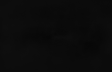
\includegraphics[width=4cm]{image/hue.png}
 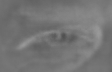
\includegraphics[width=4cm]{image/saturation.png}
 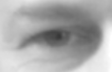
\includegraphics[width=4cm]{image/value.png}
 \caption{Décomposition du modèle HSV}
\end{figure}

solution -> calcul d'un masque pour réduire l'image pris en compte par canny
étape de construction du masque : 
\begin{itemize}
 \item égalisation des trois composante de l'image de départ
 \item passage de l'image en hsv
 \item égalisation de la composante saturation%value
 \item érosion de l'image
\end{itemize}

%test avec le value mais a mon avis c pas tres stable -> voir masqueAv.png et masqueAp.png
\begin{figure}[H]
 \center
 
\includegraphics[width=4cm]{image/resultatMasque.png}
 \caption{Résultat du masque après application du masque}
\end{figure}

saturation -> probleme sur la couleur de peau.

\begin{figure}[H]
 \center
 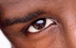
\includegraphics[width=4cm]{image/original_black.png}
 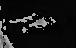
\includegraphics[width=4cm]{image/hue_black.png}
 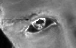
\includegraphics[width=4cm]{image/saturation_black.png}
 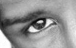
\includegraphics[width=4cm]{image/value_black.png}
 \caption{Décomposition du modèle HSV avec une couleur de peau plus foncée}
\end{figure}

\subsubsection{Le modèle YCbCr}

Nous avons testé un second modèle colorimètrique suite à l'étude des travaux de Evangelos Skodras et Nikolaos Fakotakis\cite{Skodras_2012ieee}.
En effet, leur étude montre que les différentes couleurs de peau de l'Homme ont la peu près la même valeur dans les deux
composantes de du modèle YCbCr.\\

\begin{figure}[H]
 \center
 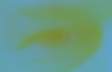
\includegraphics[width=4cm]{image/yuv_blanc.png}
 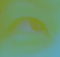
\includegraphics[width=3cm]{image/yuv_asiat.png}
 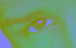
\includegraphics[width=4cm]{image/yuv_noire.png}
 \caption{Image dans le modèle YCbCr d'une personne blanche, asiatique et noire}
\end{figure}

Nous pouvons voir que quelque soit la couleur de peau des personnes étudié, la couleur
de la peau est verdâtre, mais la pupille elle reste foncée. Il est donc plus aisé de travailler 
dans ce modèle pour ne plus avoir à prendre en compte la couleur de peau. Il est possible d'obtenir
ce modèle à partir du modèle RGB grâce à la formule suivante : 
$$Y = 0.299R + 0.587 G + 0.114 B$$
$$Cb = -0.1687R - 0.3313 G + 0.5B + 128$$
$$Cr = 0.5R -0.4187G -0.0813B + 128$$

\begin{figure}[H]
 \center
 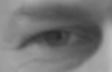
\includegraphics[width=4cm]{image/luminance.png}
 
\includegraphics[width=4cm]{image/chrominance1.png}
 
\includegraphics[width=4cm]{image/chrominance2.png}
 \caption{Décomposition du modèle YUV}
\end{figure}

\begin{figure}[H]
 \center
 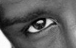
\includegraphics[width=4cm]{image/luminance_black.png}
 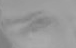
\includegraphics[width=4cm]{image/chrominance1_black.png}
 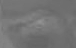
\includegraphics[width=4cm]{image/chrominance2_black.png}
 \caption{Décomposition du modèle YUV avec une couleur de peau plus foncée}
\end{figure}

\begin{figure}[H]
 \center
 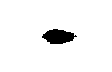
\includegraphics[width=4cm]{image/pupille.png}
 \caption{Résulata après traitement sur la chominance 1}
\end{figure}

\begin{figure}[H]
 \center
 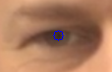
\includegraphics[width=4cm]{image/localisation1.png}
 \caption{Première localisation du centre de l'oeil avec traitement sur le modèle YUV}
\end{figure}

problème -> instable et ne fonctionnement pas sur toutes les personnes

\subsection{Détection des contours et calcul du barycentre de la forme}

\subsection{L'algorithme de Gabor}